% Chapter 6

\chapter{Implementation, Results and Discussion} % Main chapter title

\label{Chapter6} % For referencing the chapter elsewhere, use \ref{Chapter6} 

\lhead{Chapter 6. \emph{Implantation, Results and Discussion}} % This is for the header on each page - perhaps a shortened title

%----------------------------------------------------------------------------------------

\section{Introduction}
In Chapter \ref{Chapter5}, the adopted development process, the tools used and the work environment were examined in details.

In this chapter, experiments of different classification procedures, dataset 
splits and feature selection are presented. Results are introduced in section 
\ref{sec:6_results_disscusion}. The discussion and analysis of obtained results are presented in section 6.4.

\section{Implementation Details}
%==============================

\subsection{Classification Web Service implementation details}
This section will discuss the implementation details of the classification web service.


    \subsubsection{Training Phase}
    Once the user have registered in the classification web service, Smart Email will start downloading pre-classified emails from
    user email provider using IMAP protocol.

    Smart Email design described in the previous chapter is flexible and enables using different data sources,a file data source was used
    to read Enron \cite{ENRON} dataset from file system.

    Other protocols can be implemented like POP3.

    \subsubsection{Preprocessing phase}
    Smart Email uses several preprocessors on incoming emails. The following are the currently implemented preprocessors,
    the design of the Smart Email allows the addition of other preprocessors without modification to the existing code.
        \begin{description}
        \item[Stemming] Porter stemmer \cite{STEMMER} is used to stem words of email.
        \item[Stop words removal] is used to remove stop words like ("the","them",.. etc).
        \item[Lowercasing] is used to convert all words in subject and body to lowercase.
        \item[Number Normalization] is used to convert all numbers to a specific tag.
        \item[URL Normalization] is used to convert all urls into specific tags.
        \item[HTML tags remover] is used to remove html tags from emails if they exists.
        \end{description}

    \subsubsection{Classification phase}
    When a new Incoming Email is sent to the classification web service,
    the email is preprocessed as described above and features (described in details in Chapter \ref{Chapter3}
    are Extracted to build the input tuple.

    The input tuple is then given to WEKA \cite{WEKA} (Naive Bayes or SVM) classifier to 
    perform the classification. The result of the classification is then returned.

\subsection{Email monitoring web service implementation details}
    Users register in the email monitoring web service by providing user name and passwords,
    then the user can add one or more email accounts to be monitored.
    A Job runs in the background opening IMAP-IDLE connection for every user's email account.
    This job sends every new incoming email to the classification web service and
    applies the returned label to user's email.

    This web service was built using ruby on rails \cite{ROR} framework, MySql database was used
    in development environment while postgresql was used in production.


\subsection{Chrome Browser Extension implementation details}
    Chrome Extension is a client side extension for the Google chrome browser \cite{CHROME}.
    The extension injects a javascript file in the gmail web interface. The extension also manipulates
    gmail web interface HTML page by injecting a button entitled "Classify Me"
    that appears when the user selects any email to view.

    The button is injected by adding a new DOM element to the html page.The extension must waits till
    the page completely loads to do the injection.

    When the user clicks the "Classify Me" button the extension retrieves the raw email and
    builds a message using the raw email,an ajax call with the message is made to the 
    classification web service.

    The extension also detects when the user tries to manually classify an email, The extension builds
    a feedback message with the email and the correct label, then sends it to the classification 
    web service.

    To detect events like manual classification, the extension must intercepts ajax requests made by
    gmail and examines the request body.

    The Extension uses the Gmailr library \cite{GMAILR} to detect various events. The library was modified 
    to be able to detect "apply new label" event.

%--------------------------------------------------------------------------------------
\section{Results and Discussion}
\label{sec:6_results_disscusion}
\subsection{Experimental Setup}

\subsubsection{Enron Dataset \cite{ENRON}}
Enron dataset is the most popular email corpus for research. It was released during the legal investigation into the Enron corporation.
It is an invaluable dataset since it contains uncensored messages from a corporate environment. The dataset consists of employee’s email folders, so it is also an accurate depiction of how users use folders. The majority of email directories in the dataset are small, so seven users with the largest email directories are chosen for the experiments. Those seven users are chosen in many related papers (e.g. Huang, Bekkerman and McCallum, 2004\cite{RON04}). \\Statistics on the seven users are shown in table \ref{enronStatsTable}:

\begin{center}
	\centering
	\begin{table}[H]
		\begin{tabular}{ |  >{\centering} l |  >{\centering} p{1.75cm} |  >{\centering} p{1.75cm} |  >{\centering}p{1.75cm} |  >{\centering} p{1.75cm} |  >{\centering} p{1.75cm} | p{1.75cm} <{\centering} | }
		\hline

		User & Number \newline of \newline folders & Number \newline of \newline messages & Size of \newline smallest \newline folder \newline (messages) & Size of \newline largest \newline folder \newline (messages) & Size of \newline smallest \newline message \newline (words) & Size of \newline largest \newline message \newline (words) \\ \hline \hline

		Beck-s & 101 & 1971 & 3 & 166 & 45 & 2620 \\ \hline
		Farmer-d & 25 & 3672 & 5 & 1192 & 43 & 3507 \\ \hline
		Kamniski-v & 41 & 4477 & 3 & 547 & 44 & 7885 \\ \hline
		Kitchen-l & 47 & 4015 & 5 & 715 & 47 & 46296 \\ \hline
		Lokay\_m & 11 & 2489 & 6 & 1159 & 45 & 4456 \\ \hline
		Sanders\_r & 30 & 1188 & 4 & 420 & 55 & 19331 \\ \hline
		Williams-w3 & 18 & 2769 & 3 & 1398 & 49 & 2287 \\ \hline
		\hline

		\end{tabular}
	\caption{Statistics on Enron datasets after removing non-topical and small folders.}
	\label{enronStatsTable}
	\end{table}
\end{center}



\subsubsection{Experiments}
Two types of experiments are reported:

\begin{itemize}
\item Learning Curves (Timeline): A learning curve is done by calculating the accuracy of each training/test split and plotting the classification accuracy curve over the number of training messages in the splits. 

\item Feature Comparison: Different combinations of possible classification features are selected and the accuracy of each combination is plotted. Each combination is run using both Naive Bayes and SVM algorithms.
\end{itemize}

\subsubsection{Training/test Set Splits}
In practice, the dataset grows over time. So, a natural way of splitting the dataset would be based on time: train on earlier emails and test on later ones. A similar approach is employed in (Klimt and Yang, 2004)\cite{KY04}. 
The incremental time-based split is done by sorting the emails according to their time stamp, then the classifier is trained on the first N messages and tested against the following N messages, then it is trained on the first 2N messages and tested against the following N messages etc. until we cover the whole dataset. N was chosen to be 100 which is similar to experiments conducted in (Bekkerman, McCallum and Huang 2004)\cite{RON04}.

\subsection{Results}

\subsubsection{Learning Curves}
Results of the seven Enron users are presented below as the accuracy over the timeline for each user.

\begin{figure}[H]
    \begin{center}
    \subfigure[beck-s]{
        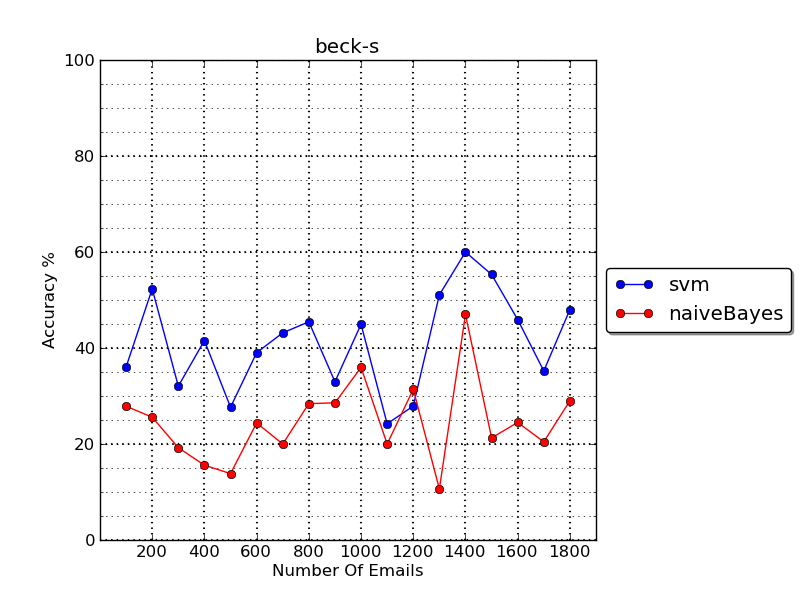
\includegraphics[scale=0.3]{beck-s.png}
    }
    \subfigure[farmer-d]{
        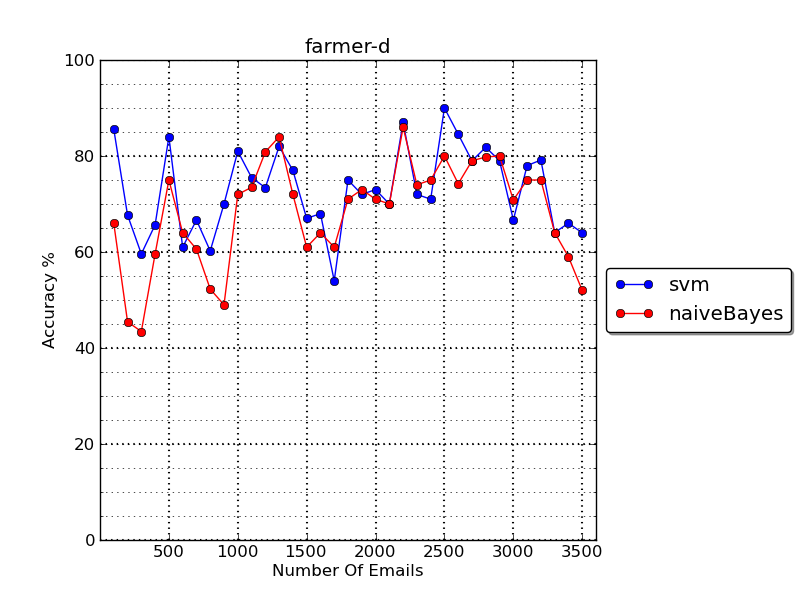
\includegraphics[scale=0.3]{farmer-d.png}
    }
    \subfigure[kamniski-v]{
        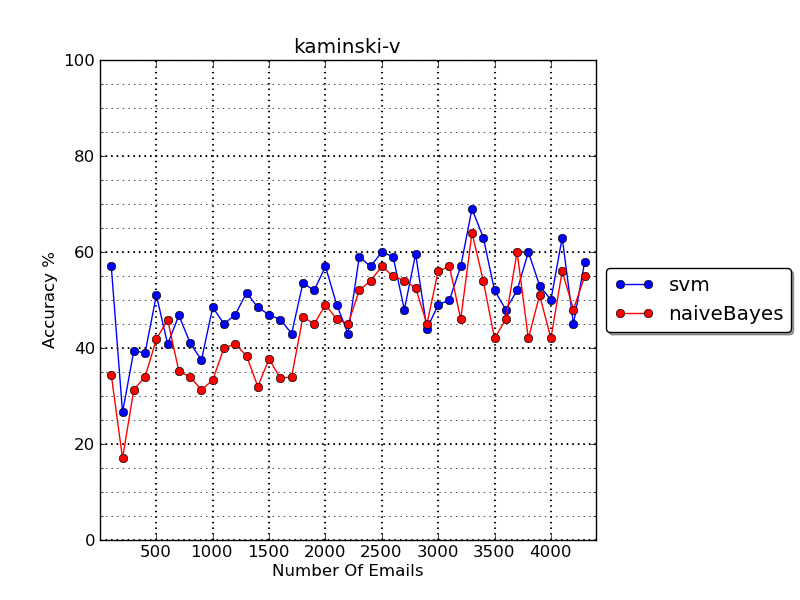
\includegraphics[scale=0.3]{kaminski-v.png}
    }
    \subfigure[kitchen-l]{
        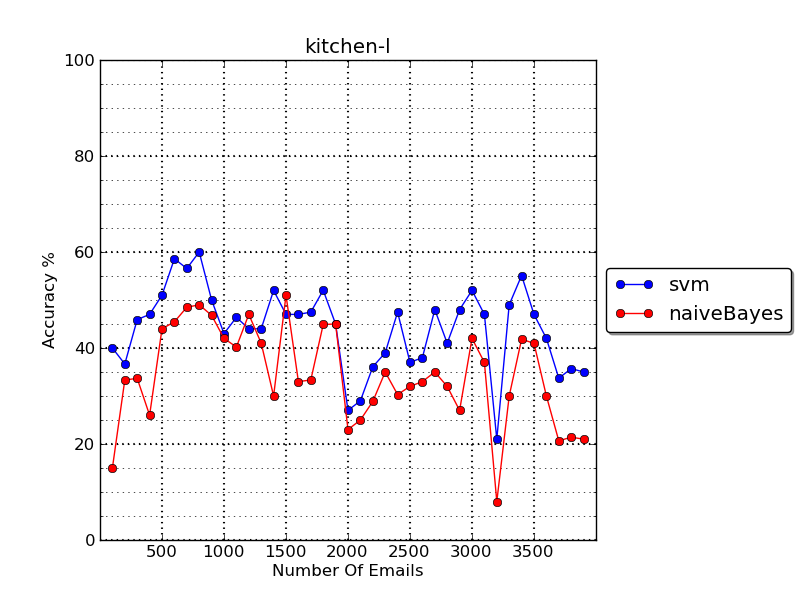
\includegraphics[scale=0.3]{kitchen-l.png}
    }
    \subfigure[lokay\_m]{
        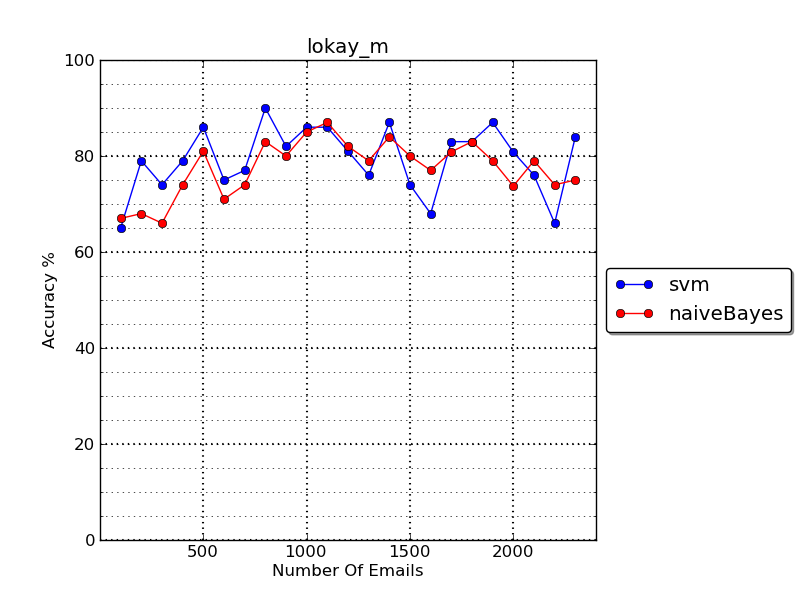
\includegraphics[scale=0.3]{lokay_m.png}
    }
    \subfigure[sanders\_r]{
        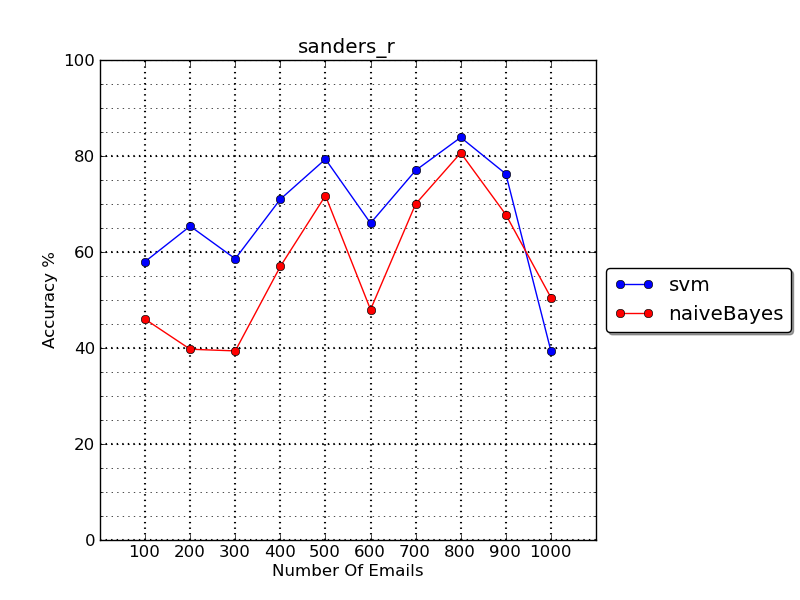
\includegraphics[scale=0.3]{sanders_r.png}
    }
    \subfigure[williams-w3]{
        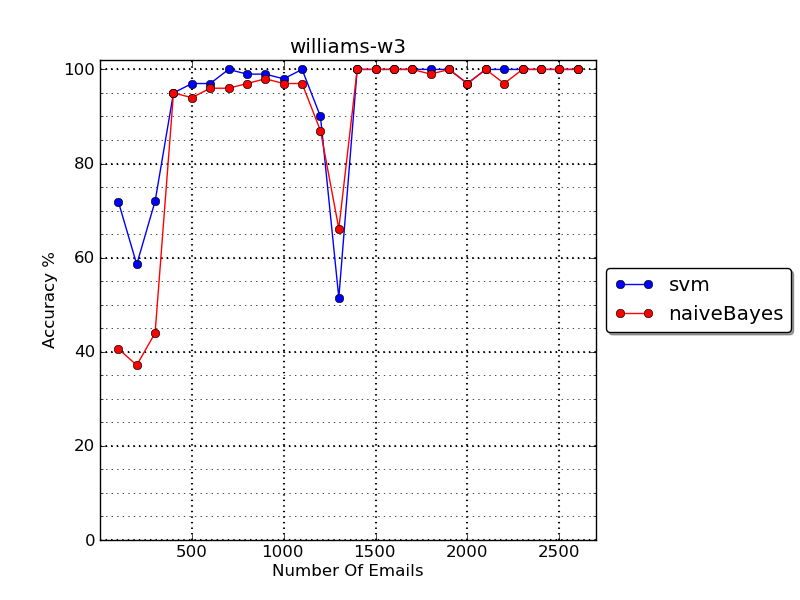
\includegraphics[scale=0.3]{williams-w3.png}
    }
    \end{center}
    \caption{Timeline results (learning curvers)}
\end{figure}

The following table is the accuracies averaged over all training/test splits for all users. It has two columns representing the two different classification algorithms: Naive Bayes and SVM.

\begin{table} [!htbp]
	\begin{center}

	    \begin{tabular}{ | l | l | l |}
	    \hline
	    User {\textbackslash}  Classifier & Naive Bayes & SVM \\ \hline
	    Beck-s & 24.65\% & 41.27\% \\ \hline
	    Farmer-d & 68.36\% & 72.87\% \\ \hline
	    Kamniski-v & 44.53\% & 50.36\% \\ \hline
	    Kitchen-l & 34.44\% & 44.15\% \\ \hline
	    Lokay\_m & 77.50\% & 79.34\% \\ \hline
	    Sanders\_r & 57.08\% & 67.49\% \\ \hline
	    Williams-w3 & 89.92\% & 93.30\% \\
	    \hline
	    \end{tabular}
	\caption{Average accuracy over all training/test splits}
	\end{center}
\end{table}

\subsubsection{Feature Comparison}
Different combinations of the features affect the accuracy of classifiers. It is not necessarily that adding a feature will improve accuracy. So, it was important to test different features combinations to select the best combination. The results of six different combinations are reported below for each user. Each combination is tested under both Naive Bayes and SVM classification algorithms.

\begin{figure}[H]
    \begin{center}
    \subfigure[beck-s]{
        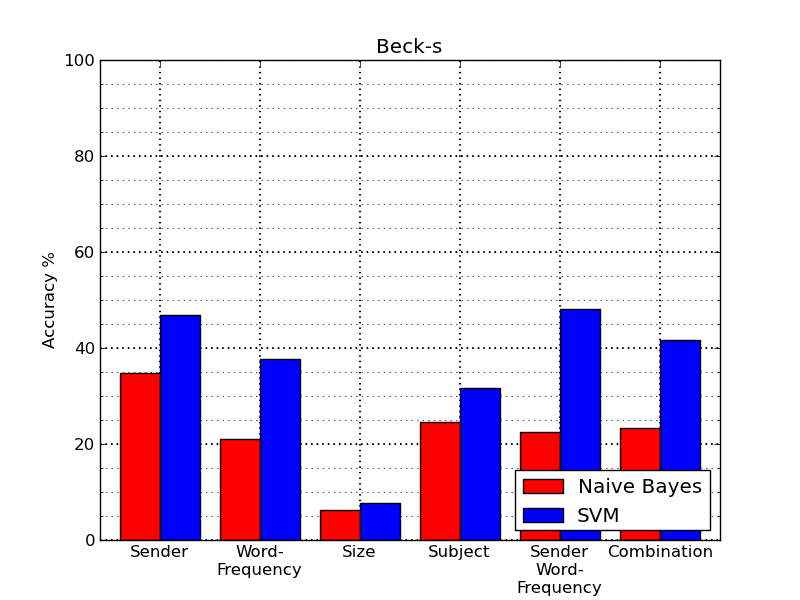
\includegraphics[scale=0.3]{F_Beck-s.png}
    }
    \subfigure[farmer-d]{
        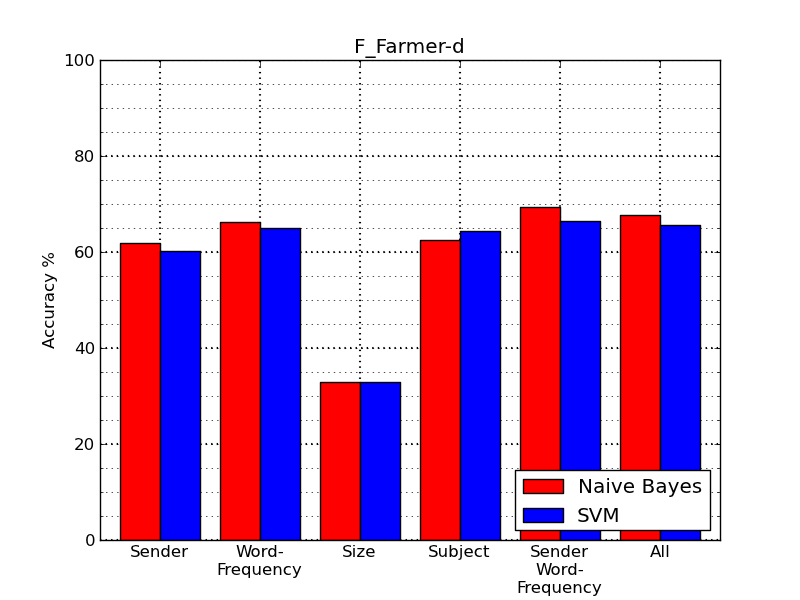
\includegraphics[scale=0.3]{F_Farmer-d.png}
    }
    \subfigure[kamniski-v]{
        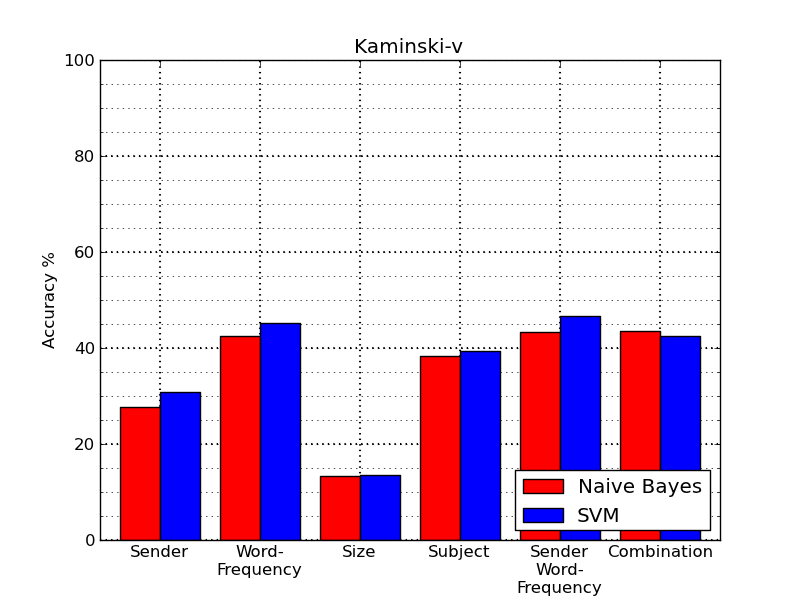
\includegraphics[scale=0.3]{F_Kaminski-v.png}
    }
    \subfigure[kitchen-l]{
        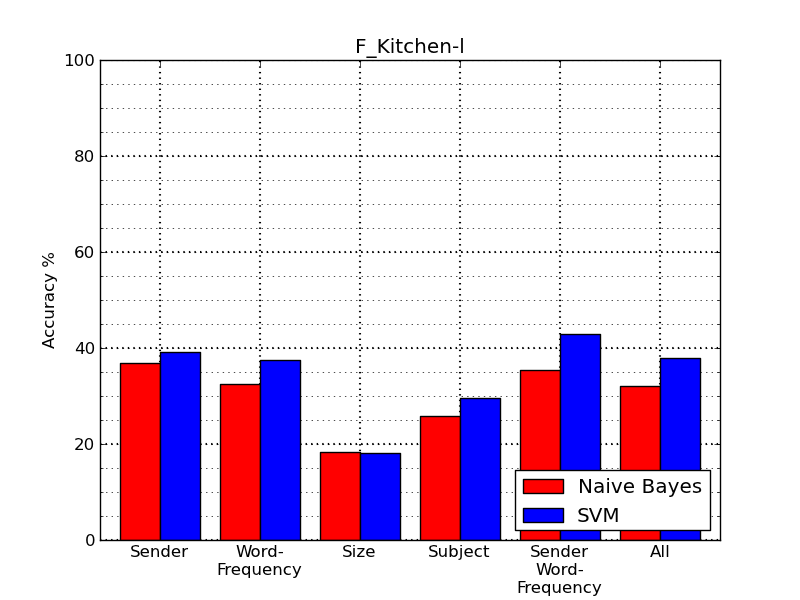
\includegraphics[scale=0.3]{F_Kitchen-l.png}
    }
    \subfigure[lokay\_m]{
        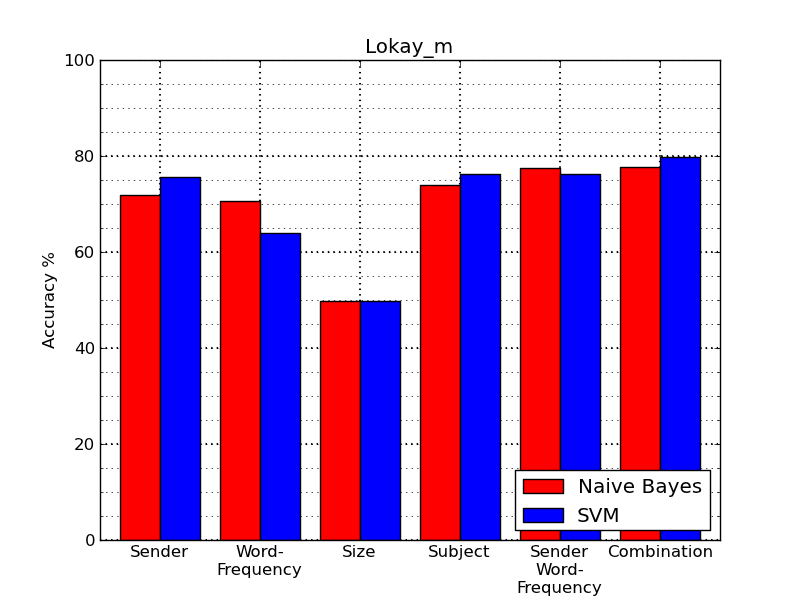
\includegraphics[scale=0.3]{F_Lokay_m.png}
    }
    \subfigure[sanders\_r]{
        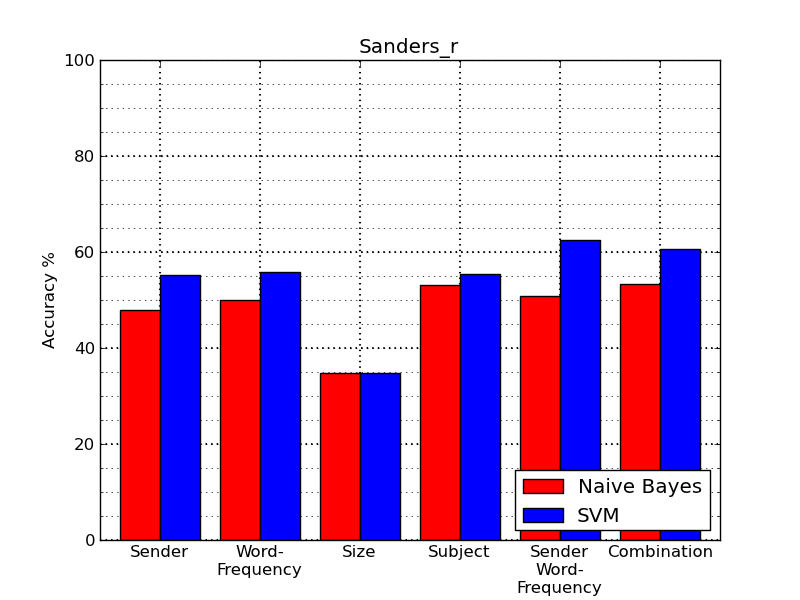
\includegraphics[scale=0.3]{F_Sanders_r.png}
    }
    \subfigure[williams-w3]{
        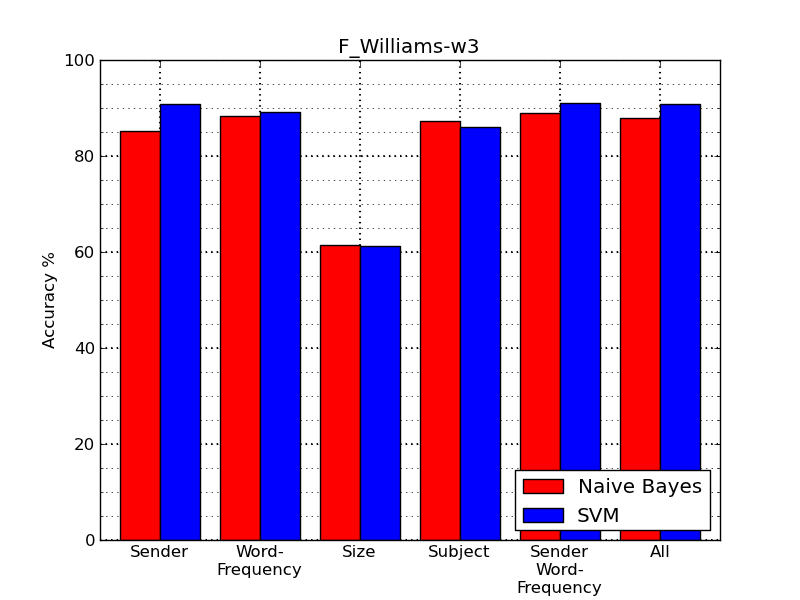
\includegraphics[scale=0.3]{F_Williams-w3.png}
    }
    \end{center}
    \caption{Results of different features combinations}
\end{figure}

%-----------------------------------------------------------------
\subsection{Discussion}
Learning curves (figure 6.1) show that SVM outperforms Naive Bayes in most of the cases. This is the expected behaviour. It is widely believed that Naive Bayes is not the best algorithm for text categorization (Dumais et al., 1998)\cite{DHS98}.
However, the results obtained doesn't reveal significance superiority of SVM over Naive Bayes. In fact, in some cases Naive Bayes was better than SVM (e.g Farmer-d feature selection figure). This is probably due to features selection and how the classifier weights each feature.


Experimental results obtained support the following observations:
\begin{itemize}
\item Accuracies are higher when the dataset has one or two dominant folders. As it can be seen from Table \ref{enronStatsTable}
 the size of the largest folder is nearly one half size of the entire dataset (e.g., users lokay\_m and williams-w3).

\item Newly created folders negatively affect the classification accuracy. If a new folder is created, the classifier trains on few emails from this folder which may not be enough to build a good classification model. (e.g see the drops in figures (6.1-f) and (6.1-g))

\item The dataset of user williams-w3 (figures (6.1-g) and (6.2-g)) is a degenerative case. It has two large folders (``bill williams iii'' and ``schedule crawler'' which contain most of the messages. This explains the high accuracy for this dataset regardless of features used.

\item Classification using the sender feature alone yields good results (figure 6.2).

\item Using both the sender feature and the bag of words (word frequency) feature achieves best results in most of the cases. Adding more features doesn't necessarily imporve the accuracy.

%TODO add more points (about feature comparison)
\end{itemize}

\section{Conclusion}
In this chapter the experimental results were presented. Analysis of the results were discussed. The results reveal the difficulty of eamil classification. Improving the accuracy is listed as a future work.

